%%%%%%%% ICLR 2027 SUBMISSION (v2.5) %%%%%%%%%%%%%%%%%%%%%%%%%%%%%%%%%%%%%%%
% "Resources, Certificates, and Limits of LLM-Guided Artifact Search"
% Compile: pdflatex main && bibtex main && pdflatex main && pdflatex main
% Review version (anonymized, line numbers). For camera-ready add
% \iclrfinalcopy below; for arXiv add \iclrarxivcopy.
%
% v2   : major revision of the ICML 2026 submission addressing both referee
%        reports (see ../icml-2026/review-icml2026.html and
%        referee-report-r2-verification.html, and response-to-reviewers.html).
% v2.5 : retitled (no longer duplicates the published blog title); ShopGym
%        decoupled (unrelated work); extended-discussion and notation
%        appendices added so the page limit never trades against
%        completeness — main text stays within 9 pp, expansions live in
%        Appendices M–N.

\documentclass{article}
\usepackage{iclr2027_conference,times}

\usepackage{microtype}
\usepackage{graphicx}
\usepackage{booktabs}
\usepackage{amsmath,amssymb,mathtools,bm}
\usepackage{amsthm}
\usepackage{tikz}
\usetikzlibrary{positioning,arrows.meta}
\usepackage{hyperref}
\usepackage{url}

% \iclrfinalcopy   % uncomment for camera-ready
% \iclrarxivcopy   % uncomment for arXiv

% ---------- theorem setup (numbered within section) ----
\theoremstyle{plain}
\newtheorem{theorem}{Theorem}[section]
\newtheorem{proposition}[theorem]{Proposition}
\newtheorem{corollary}[theorem]{Corollary}
\newtheorem{lemma}[theorem]{Lemma}
\theoremstyle{definition}
\newtheorem{definition}[theorem]{Definition}
\newtheorem{assumption}[theorem]{Assumption}
\newtheorem{example}[theorem]{Example}
\theoremstyle{remark}
\newtheorem{remark}[theorem]{Remark}

% ---------- macros ----------
\newcommand{\A}{\mathcal{A}}
\newcommand{\Y}{\mathcal{Y}}
\newcommand{\D}{\mathcal{D}}
\newcommand{\M}{\mathcal{M}}
\newcommand{\E}{\mathbb{E}}
\renewcommand{\P}{\mathbb{P}}
\newcommand{\R}{\mathbb{R}}
\newcommand{\N}{\mathbb{N}}
\newcommand{\sel}{\mathrm{sel}}
\newcommand{\len}{\ell}
\newcommand{\Fhat}{\widehat{F}}
\newcommand{\Ftil}{\widetilde{F}}
\newcommand{\eps}{\varepsilon}
\newcommand{\pgam}{p_{\gamma}}

\title{Resources, Certificates, and Limits of\\ LLM-Guided Artifact Search}

\author{Anonymous authors\\
Anonymous Institution\\
\texttt{anon.email@domain.com}}

\begin{document}

\maketitle

\begin{abstract}
A rapidly growing family of systems improves at tasks without touching model weights: an outer loop proposes edits to a textual or programmatic \emph{artifact}---a prompt, a skill document, an agent harness, a training script---scores each candidate with a noisy evaluator, and keeps what works, with a frozen large language model (LLM) as the proposal distribution. We give a single formal model containing these systems and prove that its behavior is governed by a few measurable resources: the \emph{prior mass} the proposer places on good artifacts, which controls hitting time Levin-style and whose conditioning boost $\gamma$ is estimable from samples at finite cost; the \emph{information content of feedback}, where scalar rewards can be exponentially slower than structured traces; the \emph{noise--gap ratio} of the evaluator, where a single-evaluation greedy ratchet fed pure noise reports a realized median ``improvement'' of $3.4\sigma$ after $2{,}000$ null edits while $O((\sigma^2/\Delta^2)\log(B/\delta))$ repeats per decision certify a whole run; the \emph{deceptiveness} of the landscape, where archives are exponentially faster than tolerant greedy search; and the \emph{description length} of the artifact, through an Occam bound whose U-shaped risk predicts both context collapse and validation overfitting. Beyond the per-resource analyses, we prove a \emph{composed certified-improvement theorem} that requires the assembled object: a gated loop finds and soundly certifies a near-optimal artifact in $O\big((\sigma^2/\Delta^2)\ln(B/\delta)\ln(1/\delta)/(\gamma\,q_0(G_\eps))\big)$ evaluator calls, with false rejection of true improvements an explicit slowdown factor. We map each result to documented behaviors and failures of deployed systems, ground the selection results in the archival evaluation-statistics literature, and state falsifiable scaling predictions with a pre-registered protocol for measuring $\gamma$ on a real proposer.
\end{abstract}

\section{Introduction}
\label{sec:intro}

The dominant formal account of machine learning is gradient-based: define a differentiable loss, follow its gradient in weight space. Yet many striking recent gains in LLM-based systems involve no weight updates at all. GEPA evolves prompts by reflecting on execution traces and reports outperforming the RL algorithm GRPO with up to $35\times$ fewer rollouts \citep{agrawal2025gepa}; Meta-Harness rewrites the scaffolding code around a frozen model and beats hand-built context management \citep{lee2026metaharness}; SkillOpt edits a skill document under held-out acceptance tests \citep{yang2026skillopt}; AlphaEvolve and FunSearch evolve programs against machine-checkable evaluators and produce new mathematics \citep{novikov2025alphaevolve,romeraparedes2024funsearch}; Karpathy's \emph{autoresearch} loop edits a real training codebase overnight \citep{karpathy2026autoresearch}; Heuristic Learning patches executable heuristics from replayed failures \citep{weng2026hl}; the Darwin G\"odel Machine and ADAS search over agent designs themselves \citep{zhang2025dgm,hu2025adas}.

Each system was presented with its own vocabulary---reflection, evolution, context engineering, self-improvement---and each paper's analysis, where present, is empirical. This leaves basic questions open. Why are these loops so sample-efficient when classical program search is hopeless? When does a scalar reward suffice and when are traces necessary? Why do noisy single evaluations produce celebrated improvements that later fail to replicate---a failure mode documented for a decade in the evaluation-statistics literature \citep{henderson2018matters,dodge2019show,agarwal2021precipice} and recently relived by autonomous research loops? Why do greedy prompt optimizers overfit their validation sets? Why do archives and Pareto frontiers keep appearing in independently developed systems?

\textbf{This paper.} We answer these questions in a single model. An \emph{artifact-search system} (Definition~\ref{def:as}) is a tuple $(\A, F, q, \sel, \M)$: a countable space of textual/programmatic artifacts, a noisy evaluator, an LLM proposal kernel conditioned on execution feedback and memory, a selection rule, and an accumulating history. Learning updates the artifact; the weights never move. We prove:
\textbf{(1) Prior mass governs hitting time, and the boost is measurable} (\S\ref{sec:prior}): expected proposals to an $\eps$-good artifact equal the inverse of the proposer's mass on the good set, with trace-conditioning a multiplicative boost $\gamma$ (Theorem~\ref{thm:hitting}; Proposition~\ref{prop:hitlower})---and $\gamma$ is not a free parameter: Proposition~\ref{prop:gammaest} certifies the plug-in estimator at $K = O(\ln(1/\delta)/(\eta^2 q_{\min}^2))$ verified proposals (protocol in Appendix~\ref{app:protocol}).
\textbf{(2) Feedback information separates learning rates} (\S\ref{sec:feedback}): binary success feedback needs $\Omega(2^L)$ queries on $L$-bit classes where first-error feedback needs $\le L$ (Theorem~\ref{thm:separation}; transcript bound, Theorem~\ref{thm:fano})---a worst-case companion to \citet{xu2025llf}.
\textbf{(3) Noise makes greedy ratchets unsound, quantifiably} (\S\ref{sec:selection}): a single-evaluation ratchet on pure-noise edits reports a diverging best $\E[m_t] \le \sigma\sqrt{2\ln t}$ (tight for Gaussians) while accepting $H_t = \ln t + O(1)$ null edits (Theorem~\ref{thm:ratchet}); $N = O((\sigma^2/\Delta^2)\log(B/\delta))$ repeats per decision certify a whole $B$-step run (Proposition~\ref{prop:repeats}, Corollary~\ref{cor:budget}).
\textbf{(4) Deception separates greedy from archive selection} (\S\ref{sec:selection}): on an explicit landscape with a \emph{unique} optimum, strict greedy never arrives, tolerant greedy needs $\exp(\Omega(k))$ steps, an archive arrives in $O(k^2)$ (Theorem~\ref{thm:deception})---the formal content of GEPA's Pareto sets, ADAS's archives, the DGM's lineages.
\textbf{(5) The resources compose} (\S\ref{sec:composition}): the central new result, Theorem~\ref{thm:composed}, couples prior mass, noise, and gated selection---under a margin condition a gated loop makes \emph{no} false accept and certifies an $\eps$-good artifact in $O\big((\sigma^2/\Delta^2)\ln(B/\delta)\ln(1/\delta)/(\gamma q_0(G_\eps))\big)$ evaluator calls, false-reject slowdown explicit.
\textbf{(6) Description length controls generalization} (\S\ref{sec:compression}): an Occam bound yields a U-shaped risk in artifact length explaining both \emph{context collapse} and validation overfitting (Theorem~\ref{thm:occam}, Corollary~\ref{cor:ushape}).
\textbf{(7) Proxy gaps bound the enterprise} (\S\ref{sec:limits}): measured progress transfers up to twice the bias sup-norm, selection harvests bias at the optimizer's-curse rate $\sigma_b\sqrt{2\ln m}$, and an editable evaluator voids every nonvacuous transfer guarantee via an in-model construction (Proposition~\ref{prop:goodhart}).

Sections~\ref{sec:experiments}--\ref{sec:related} provide simulations (each arm an executed algorithm) and situate the framework; proofs are in the appendices. Our aim follows \citet{bowling2023settling}: not to introduce a new algorithm, but to make precise what a fast-moving empirical literature is doing, so that its successes and failures become predictions rather than surprises---falsifiably so (\S\ref{sec:discussion}).

\section{One Loop, Many Names: the Formal Model}
\label{sec:model}

\begin{figure}[t]
\centering
\resizebox{0.5\textwidth}{!}{%
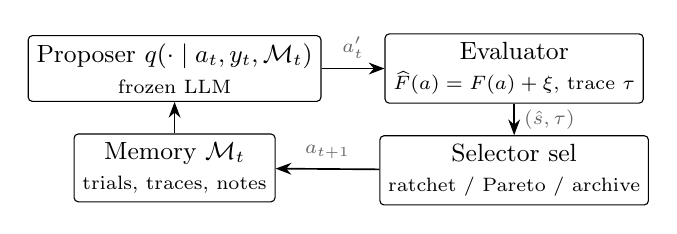
\begin{tikzpicture}[
  node distance=4mm and 8mm,
  box/.style={draw, rounded corners=1.5pt, align=center, inner sep=3pt, font=\small},
  lab/.style={font=\scriptsize\itshape, text=black!60},
  arr/.style={-{Stealth[length=2mm]}, semithick}
]
\node[box] (prop) {Proposer $q(\cdot \mid a_t, y_t, \M_t)$\\ \scriptsize frozen LLM};
\node[box, right=of prop] (eval) {Evaluator\\ \scriptsize $\Fhat(a) = F(a) + \xi$, trace $\tau$};
\node[box, below=of eval] (sel) {Selector $\sel$\\ \scriptsize ratchet / Pareto / archive};
\node[box, below=of prop] (mem) {Memory $\M_t$\\ \scriptsize trials, traces, notes};
\draw[arr] (prop) -- node[lab, above] {$a'_{t}$} (eval);
\draw[arr] (eval) -- node[lab, right] {$(\hat{s}, \tau)$} (sel);
\draw[arr] (sel) -- node[lab, above] {$a_{t+1}$} (mem);
\draw[arr] (mem) -- node[lab, right] {} (prop);
\end{tikzpicture}%
}
\caption{The artifact-search loop. Weights are frozen everywhere; learning is the trajectory $a_0, a_1, \dots$ through artifact space (Table~\ref{tab:systems}).}
\label{fig:loop}
\end{figure}

\begin{definition}[Artifact-search system]
\label{def:as}
An \emph{artifact-search system} is a tuple $\mathcal{S} = (\A, F, q, \sel, \M)$ where
(i) $\A$ is a countable set of \emph{artifacts} (finite strings: prompts, skill documents, programs, harness code);
(ii) $F : \A \to [0,1]$ is the \emph{true score}, $F(a) = \E_{z \sim \D}[s(a, z)]$ for a task distribution $\D$ and bounded per-instance score $s$, accessed only through noisy evaluations $\Fhat$ and through \emph{feedback} $y \in \Y$ (a scalar, a trace, an error message, a video);
(iii) $q(\cdot \mid a, y, \M)$ is the \emph{proposer}, a fixed conditional distribution over $\A$ realized by a frozen LLM prompted with the current artifact, feedback, and memory;
(iv) $\sel$ is a \emph{selection rule} mapping evaluated candidates to the retained state (a single incumbent, a Pareto set, an archive, a lineage);
(v) $\M_t$ is accumulated history.
A \emph{run} is the induced stochastic process $a_0, a_1, \ldots$; for $\eps \ge 0$ the \emph{good set} is $G_\eps = \{a : F(a) \ge \sup_{a'} F(a') - \eps\}$, and the \emph{hitting time} is $T = \min\{t : a_t \in G_\eps\}$.
\end{definition}

The definition is deliberately minimal:\footnote{On the noise model: $F$ is bounded in $[0,1]$, but the evaluation noise $\xi$ in $\Fhat = F + \xi$ is $\sigma$-subgaussian and may be unbounded (\S\ref{sec:selection})---the standard idealization for per-instance score averages; only tail bounds on $\xi$ are used. Where per-instance boundedness matters (\S\ref{sec:compression}), we use it explicitly.\label{fn:noise}} the systems in Table~\ref{tab:systems} differ in engineering but not in type. Learning happens \emph{in artifact space}; the gradient-trained model appears only as the fixed kernel $q$. Three structural facts drive everything that follows: $\A$ is discrete and enormous, so all guarantees must come from where $q$ puts its mass (\S\ref{sec:prior}); the loop's only contact with the task is the feedback channel $\Y$, which rate-limits learning (\S\ref{sec:feedback}); and $\Fhat$ is noisy and expensive, so selection is statistics, not bookkeeping (\S\ref{sec:selection})---constraints that bind \emph{simultaneously}, which is what \S\ref{sec:composition} quantifies.

\begin{table}[t]
\caption{Deployed systems as artifact-search systems (citations in \S\ref{sec:intro} and Appendix~\ref{app:mapping}; sc.\ = scalar score, tr.\ = execution trace). Sources marked $^\dagger$ are informal (blog posts or code repositories) rather than archival; we use them as illustrations, never as the sole support of a claim.}
\label{tab:systems}
\vskip 0.05in
\centering
\footnotesize
\begin{tabular}{@{}llll@{}}
\toprule
System & Artifact $\A$ & Feedback $\Y$ & $\sel$ \\
\midrule
GEPA & prompts & sc.\ + tr. & instance-Pareto \\
SkillOpt & skill doc & sc.\ + tr. & gated ratchet \\
ACE & context/playbook & tr. & curated incumbent \\
Meta-Harness & harness code & sc.\ + raw history & ratchet \\
autoresearch$^\dagger$ & training code & sc.\ (noisy) & greedy ratchet \\
Heuristic Learning$^\dagger$ & heuristic code & tr.\ (logs, video) & gated ratchet \\
ADAS / DGM & agent programs & sc.\ + tr. & archive / lineage \\
FunSearch / AlphaEvolve & programs & sc.\ (verified) & island archive \\
OPRO / APE / PromptBreeder & prompts & sc. & population \\
Voyager & skill library & tr. & additive library \\
\bottomrule
\end{tabular}
\vskip -0.1in
\end{table}

\paragraph{Where the inner magic lives.}
Our results treat $q$ as a black-box measure. Why a frozen LLM is a \emph{useful} measure is the in-context-learning literature's question: conditioning behaves like implicit Bayesian inference \citep{xie2022explanation, akyurek2023what}, and trained transformers emulate learning algorithms in context \citep{vonoswald2023transformers, garg2022what}. We import this as licence for the assumption that feedback conditioning \emph{increases} $q(G_\eps)$ (Assumption~\ref{ass:boost})---made falsifiable rather than free by Proposition~\ref{prop:gammaest} and Appendix~\ref{app:protocol}.

\paragraph{Relation to classical objects.}
With $q$ fixed and $\Y$ trivial, Definition~\ref{def:as} is randomized program search, and Levin's universal search \citep{levin1973universal, solomonoff1964formal} with its descendants \citep{schmidhuber2004oops, schmidhuber1997shifting, hutter2005universal, achille2025universal} applies verbatim; with $\A$ a population and $\sel$ an archive, it is quality-diversity evolution \citep{lehman2011abandoning, mouret2015illuminating}; with $\sel$ statistical and $\Fhat$ noisy, it is best-arm identification \citep{maron1994hoeffding, evendar2006action, karnin2013almost, li2017hyperband}. Our contribution is to make the translations exact, extract the quantitative consequences for the LLM-era instantiations, and prove one statement (Theorem~\ref{thm:composed}) that needs all the parts at once.

\section{Resource I: Prior Mass}
\label{sec:prior}

No search rule can beat uniform enumeration on average over all problems \citep{wolpert1997no}; concretely, for a target placed \emph{uniformly at random} in a space of size $|\A|$---the hypothesis of Theorem~\ref{thm:separation}(i) below---every algorithm has expected hitting time $(|\A|+1)/2$. Whatever makes artifact search tractable must be alignment between proposer and problem; the following theorem says this alignment is one number.

\begin{assumption}[Trace boost]
\label{ass:boost}
There exist $\gamma_t \ge 0$ such that, almost surely over histories, the conditioned proposer satisfies $q(G_\eps \mid a_t, y_t, \M_t) \ge \gamma_t\, q_0(G_\eps)$, where $q_0$ is the unconditioned (cold) proposal distribution.
\end{assumption}

\begin{theorem}[Hitting time = inverse prior mass]
\label{thm:hitting}
Let proposals $a'_1, a'_2, \ldots$ be drawn from the system's proposer and let $T$ be the first time $a'_t \in G_\eps$.
\begin{enumerate}\itemsep1pt
\item[(i)] If proposals are i.i.d.\ from $q$ with $p \coloneqq q(G_\eps) > 0$, then $\E[T] = 1/p$, and $T \le \ln(1/\delta)/p$ with probability $\ge 1-\delta$.
\item[(ii)] If each proposal costs compute $c(a)$ with $\bar{c} = \E_{a \sim q}[c(a)] < \infty$, the expected total compute is $\E\big[\sum_{t \le T} c(a'_t)\big] = \bar{c}/p$.
\item[(iii)] Under Assumption~\ref{ass:boost} with $\gamma_t \ge \gamma > 0$ for all $t$, $\E[T] \le 1/(\gamma\, q_0(G_\eps))$, and more generally $\E[T] \le t_0 + 1/(\gamma\, q_0(G_\eps))$ if the bound holds only for $t \ge t_0$.
\end{enumerate}
\end{theorem}

\begin{proposition}[Lower bound]
\label{prop:hitlower}
If instead $q(G_\eps \mid \cdot) \le \bar{q}$ almost surely at every step, then $\E[T] \ge 1/(2\bar{q}) - 1$.
\end{proposition}

\begin{remark}[Misleading feedback; exact-mass version]
\label{rem:misleading}
If the conditional good-set mass \emph{equals} $\gamma\, q_0(G_\eps)$ at every step, $T$ is geometric and $\E[T] = 1/(\gamma\, q_0(G_\eps))$ exactly: conditioning with $\gamma < 1$ is strictly slower than cold sampling. Under only the one-sided hypothesis of Proposition~\ref{prop:hitlower}, the conclusion $\E[T] > 1/q_0(G_\eps)$ follows for $\gamma < 1/\big(2(1 + q_0(G_\eps))\big)$, but not for all $\gamma < 1$.
\end{remark}

\begin{proposition}[The boost is estimable]
\label{prop:gammaest}
Suppose membership in a good set $G$ is decidable by a verifier and $q_0(G), q_\tau(G) \ge q_{\min} > 0$, where $q_\tau$ is the trace-conditioned proposer. Draw $K$ i.i.d.\ proposals from each and let $\hat\gamma = \hat{q}_\tau(G)/\hat{q}_0(G)$ be the plug-in ratio of empirical pass rates. For any $\eta \in (0,1]$, $\delta \in (0,1)$: if $K \ge \tfrac{9}{2\, q_{\min}^2\, \eta^2} \ln \tfrac{4}{\delta}$, then with probability $\ge 1-\delta$, $(1-\eta)\,\gamma \le \hat\gamma \le (1+\eta)\,\gamma$, where $\gamma = q_\tau(G)/q_0(G)$.
\end{proposition}

Proofs are in Appendix~\ref{app:prior}; (ii) is Wald's identity \citep{wald1944cumulative}, and (i)+(iii) form an adaptive analogue of Levin's bound \citep{levin1973universal}. Proposition~\ref{prop:gammaest} makes Assumption~\ref{ass:boost} an empirical claim rather than a relabeling: the boost is certifiable from $O(\ln(1/\delta)/q_{\min}^2)$ verified proposals per condition, and Appendix~\ref{app:protocol} turns this into a concrete experiment (sample patches from a frozen model with and without the execution trace in context, against a held-out verifier; report the Wilson-interval ratio). Three readings matter. \emph{Pretraining buys $q_0(G_\eps)$:} the cold mass a frontier model puts on ``useful edits to this artifact'' is what moved between 2017-era neural program search \citep{zoph2017nas} and FunSearch---the search barely changed; the prior did \citep[cf.][]{achille2025universal}. \emph{Traces buy $\gamma_t$:} a proposer that reads a stack trace concentrates $q$ on the edits consistent with it; \S\ref{sec:feedback} bounds the multiplier by the information in $y$. Run backward, the mechanism is a warning: misleading feedback slows search below cold sampling---exactly so under Remark~\ref{rem:misleading}'s exact-mass reading, via Proposition~\ref{prop:hitlower} once $\gamma$ is small---a regime reported where traces are uninformative, e.g.\ sparse-reward exploration \citep{weng2026hl}. \emph{Reuse compounds the prior:} adding solved-task artifacts to $\M$ re-weights $q_0$ for later problems---incremental bias shift \citep{schmidhuber1997shifting}.

\section{Resource II: Feedback Information}
\label{sec:feedback}

Fix the prior; what does richer feedback buy? Model one round as: the learner proposes $a \in \A$, and a feedback oracle returns $y = \phi(a, a^*) \in \Y$, where $a^*$ is an unknown target artifact and $\phi$ the feedback protocol. Identification of $a^*$ is the cleanest stand-in for ``learning the task''; richer settings reduce to it locally.

\begin{theorem}[Transcript bound]
\label{thm:fano}
Let $\A^* \subseteq \A$ with $|\A^*| = 2^L$ and let $a^*$ be uniform on $\A^*$. Any (possibly randomized) algorithm that identifies $a^*$ within $T$ rounds with probability $\ge 1/2$, using feedback alphabet $\Y$ with $|\Y| \ge 2$, satisfies
$T \;\ge\; (L - \log_2 6) / \log_2 |\Y|$.
\end{theorem}

\begin{theorem}[Exponential separation]
\label{thm:separation}
Let $\A^* = \{0,1\}^L$ and $a^*$ uniform.
\begin{enumerate}\itemsep1pt
\item[(i)] \textbf{Scalar success reward} ($\phi = \mathbf{1}\{a = a^*\}$): every algorithm has $\E[T] \ge (2^L + 1)/2$.
\item[(ii)] \textbf{First-error feedback} ($\phi$ = index of the first coordinate where $a$ disagrees with $a^*$): a deterministic algorithm identifies $a^*$ in at most $L$ rounds.
\item[(iii)] \textbf{Distance feedback} ($\phi$ = Hamming distance): $L + 1$ rounds suffice.
\end{enumerate}
\end{theorem}

In (ii), ``identifies'' means the algorithm \emph{knows} $a^*$ after at most $L$ responses; if the protocol additionally requires observing the success response, one confirming query is added (worst case $L+1$)---the convention our simulation adopts, whence the realized average $L/2+1$ in Figure~\ref{fig:feedback}.

The gap between (i) and (ii) is $2^L$ vs.\ $L$: \emph{exponential}, and not an artifact of alphabet size---first-error feedback uses an alphabet of size $L{+}1$, only logarithmically wider by Theorem~\ref{thm:fano}, yet exponentially more \emph{usable} because each response certifies a prefix and names a fault: precisely the structure of a stack trace, a failed unit test with its name, or a judge critique that says \emph{where} the rollout went wrong. The general theory of such speedups is the transfer eluder dimension of \citet{xu2025llf}, with benchmarks in \citet{cheng2023llfbench}; Theorem~\ref{thm:separation} is the minimal worst-case example one can keep in one's head \citep{shannon1948mathematical, cover2006elements}. Through this lens, GEPA's reported advantage over GRPO at matched rollout budgets \citep{agrawal2025gepa} is the prediction of (i)-vs-(ii) for systems that read traces versus systems that collapse rollouts to scalars---a comparison recurring in TextGrad, Trace, Reflexion, and Meta-Harness's raw histories \citep{yuksekgonul2024textgrad, cheng2024trace, shinn2023reflexion, lee2026metaharness}. Conversely, scalar-only loops are not doomed, merely slow by the measure of Theorem~\ref{thm:fano}, which is why they appear where evaluation is verified and cheap (FunSearch's millions of scalar-scored calls; \citealp{romeraparedes2024funsearch}).

\section{Selection: Noise and Deception}
\label{sec:selection}

The selector sees neither $F$ nor $a^*$; it sees $\Fhat = F + \xi$ under an evaluation budget. Two independent hazards arise: \emph{statistical} (noise creates fictitious progress) and \emph{geometric} (real progress requires descending).

\subsection{The Ratchet Illusion}
\label{sec:ratchet}

Model a worst case that is also the common case at the frontier of a tuned system: a stream of \emph{null edits}, each with true gain $0$, evaluated once with $\sigma$-subgaussian noise. The greedy single-evaluation ratchet is the rule of naive prompt hill-climbing and---as informally documented---of autoresearch \citep{karpathy2026autoresearch}.

\begin{theorem}[Ratchet illusion]
\label{thm:ratchet}
Let $\hat{s}_1, \dots, \hat{s}_t$ be the measured scores of $t$ null edits, i.i.d.\ $\sigma$-subgaussian, and let $m_t = \max_{i \le t} \hat{s}_i$ be the reported best. Adopt the \emph{empty-incumbent} convention: the first candidate is accepted unconditionally, and candidate $i$ is accepted iff $\hat{s}_i > \max_{j<i} \hat{s}_j$.
\begin{enumerate}\itemsep1pt
\item[(i)] $\E[m_t] \le \sigma\sqrt{2 \ln t}$, and for Gaussian noise $\E[m_t] \ge (1 - o(1))\,\sigma\sqrt{2\ln t}$: the reported improvement diverges although every artifact is worthless.
\item[(ii)] The expected number of accepted edits is $H_t = \sum_{i \le t} 1/i = \ln t + O(1)$, independent of $\sigma$. (Under a \emph{measured-incumbent} convention---baseline $\hat{s}_0$ drawn first---the count is $H_{t+1} - 1$, an $O(1)$ difference.)
\end{enumerate}
\end{theorem}

\begin{proposition}[Cost of a sound decision]
\label{prop:repeats}
Let evaluations be $\sigma$-subgaussian about their means.
\begin{enumerate}\itemsep1pt
\item[(i)] \textbf{Two-sided gate.} To distinguish a true gain $\Delta$ from a null edit with both error probabilities $\le \delta$, it suffices to average $N \ge (16\sigma^2/\Delta^2)\ln(1/\delta)$ fresh evaluations of the candidate and of the incumbent and accept iff the measured gain exceeds $\Delta/2$.
\item[(ii)] \textbf{Lower bound.} Any rule with both errors $\le \delta$ requires $N \ge (2\sigma^2/\Delta^2)\ln\!\big(1/(4\delta)\big)$.
\item[(iii)] \textbf{One-sided gate.} Against an incumbent whose mean is known, $N \ge (8\sigma^2/\Delta^2)\ln(1/\delta)$ evaluations of the candidate alone suffice (accept iff the candidate's mean exceeds the incumbent mean by $\Delta/2$).
\end{enumerate}
\end{proposition}

\begin{corollary}[Certifying a whole run]
\label{cor:budget}
A $B$-decision loop applying Proposition~\ref{prop:repeats} with $\delta' = \delta/B$ makes no false accept during the entire run with probability $\ge 1 - \delta$, at per-decision cost (i) $N = \lceil (16\sigma^2/\Delta^2) \ln(B/\delta) \rceil$ two-sided, or (ii) $N = \lceil (8\sigma^2/\Delta^2) \ln(B/\delta) \rceil$ against a known incumbent mean: soundness costs only a $\log B$ factor.
\end{corollary}

\begin{figure}[!t]
\centering
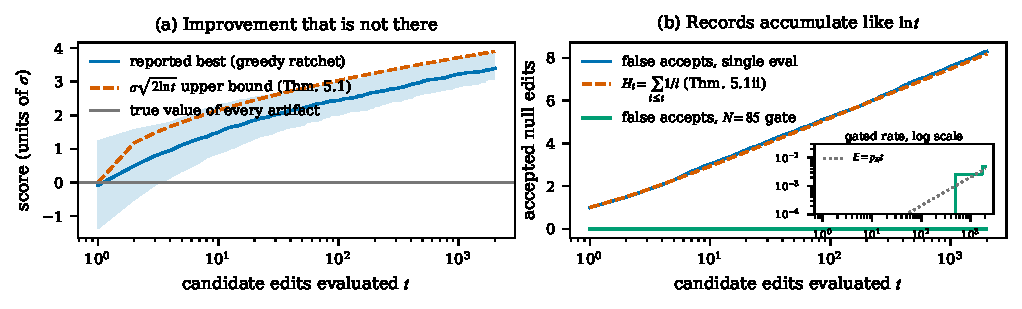
\includegraphics[width=0.94\textwidth]{figures/fig_ratchet.pdf}
\caption{The ratchet illusion (Theorem~\ref{thm:ratchet}, Corollary~\ref{cor:budget}). Null edits, $\sigma = 1$, 400 runs, seed committed. \textbf{(a)} Reported best of a single-evaluation greedy ratchet (median, 10--90\% band) against the $\sigma\sqrt{2\ln t}$ \emph{upper bound}: realized median $3.39\sigma$ at $t{=}2000$ vs.\ the bound's $3.90\sigma$ (the gap is the second-order extreme-value correction); every artifact's true value is $0$. \textbf{(b)} Accepted null edits track $H_t$ ($8.30$ simulated vs.\ $8.18$); the $N{=}85$ gate (Corollary~\ref{cor:budget}(ii) at $B{=}2000$, $\delta{=}0.05$, $\Delta{=}\sigma$) yields 2 false accepts across $8 \times 10^5$ gated decisions---rate $0.005$/run, within the $\delta = 5\%$ certificate, consistent with the Poisson prediction $1.61$ (inset, log scale, vs.\ $\E = p_N t$, $p_N \approx 2 \times 10^{-6}$).}
\label{fig:ratchet}
\end{figure}

Theorem~\ref{thm:ratchet} is extreme-value theory \citep{boucheron2013concentration} plus the classical record-counting identity; Proposition~\ref{prop:repeats} is a two-point testing bound \citep{tsybakov2009introduction, hoeffding1963probability}. The practical content is blunt: a loop making $B = 2000$ single-evaluation decisions at $\sigma = \Delta$ reports meaningful-looking progress on pure noise---a realized median of $3.4\sigma$ at $t = 2000$, climbing toward the $\sigma\sqrt{2\ln t} = 3.9\sigma$ ceiling---and accepts $\approx 8.2$ null edits ($H_{2000} \approx 8.18$); the \emph{same} loop gated with $N = 85$ repeats per decision (Corollary~\ref{cor:budget}(ii)) is sound for the whole run at the 5\% level (Figure~\ref{fig:ratchet}). The phenomenon has an archival evidence base predating LLM loops: expected-maximum reporting across tuning trials inflates exactly as Theorem~\ref{thm:ratchet}(i) prescribes, which is why \citet{dodge2019show} demand expected-validation-performance curves; few-seed point estimates routinely reverse conclusions in deep RL \citep{henderson2018matters}; and interval-based aggregation of precisely the Corollary~\ref{cor:budget} type is the remedy of \citet{agarwal2021precipice}. The recent autoresearch episode---a circulated ``53\% speedup'' from single 5-minute evaluations that did not survive re-evaluation, alongside an 11\% gain that did (informally documented; \citealp{karpathy2026autoresearch})---is the same theorem executed in public; we cite it as illustration, not evidence. Racing and successive halving spend the $N$ evaluations adaptively \citep{maron1994hoeffding, karnin2013almost, li2017hyperband}.

\subsection{Deception: when descending is necessary}
\label{sec:deception}

Noise aside, greedy selection fails where the path to the optimum passes through worse artifacts---\emph{deception} in the evolutionary-computation sense \citep{lehman2011abandoning, stanley2015greatness}.

\begin{theorem}[Deception separation]
\label{thm:deception}
Let $\A = \{0, 1, \dots, 2k\}$ be a chain with $f(i) = k - i$ on $[0, k]$ and $f(i) = 2(i - k)$ on $[k, 2k]$, so that $f(2k) = 2k > k = f(0)$ and the global optimum $2k$ is \emph{unique}, while the slope on $[0,k]$ points away from it. Each step proposes a uniformly random element of $\{i-1, i+1\}$; out-of-range proposals are rejected (the walk stays). Start at $0$.
\begin{enumerate}\itemsep1pt
\item[(i)] \textbf{Strict greedy} (accept only improvements) never reaches $2k$: it halts at $0$, an artifact whose score is $k$ below the optimum, with hitting time $\infty$.
\item[(ii)] \textbf{Tolerant greedy} (accept worsening moves with probability $\eps \in (0,1)$) has $\E[T] \ge 2\,\eps^{-k}$.
\item[(iii)] \textbf{Archive search} (keep all visited artifacts; expand a uniformly random archive member by a random neighbor; ignore $f$ entirely until the end) has $\E[T] \le 4k(2k+1) = O(k^2)$.
\end{enumerate}
\end{theorem}

The proof of (ii) is a birth--death drift computation; (iii) is a frontier argument (Appendix~\ref{app:deception}); the acceptance dynamics, hence the exact expectations, are unchanged by the asymmetric ascent slope, whose only role is to make the optimum unique. The theorem licenses a unification practitioners reached by convergent evolution: GEPA's per-instance Pareto frontier keeps candidates best at \emph{something} even when worse on average \citep{agrawal2025gepa}; ADAS retains an archive of all discovered agents \citep{hu2025adas}; the DGM maintains an expanding lineage \citep{zhang2025dgm}; FunSearch's islands are archives with migration \citep{romeraparedes2024funsearch}---all mechanisms buying polynomial valley-crossing at the price of evaluating diverse, currently-worse artifacts, MAP-Elites logic \citep{mouret2015illuminating} transplanted to text space. The theorem also delimits the claim: on deception-free landscapes greedy is optimal among these rules, which is why bounded, well-gated ratchets (SkillOpt, Heuristic Learning) thrive on tasks where each failure names its own fix.

\section{Composition: a Certified-Improvement Theorem}
\label{sec:composition}

Each result so far isolates one resource in a deliberately minimal sub-model; a fair criticism of any dictionary is that nothing yet \emph{requires} the assembled object. The following theorem does: it runs the \S\ref{sec:prior} proposer against the \S\ref{sec:ratchet} evaluator under the Corollary~\ref{cor:budget} gate, accounting for their interaction---the gate that blocks fictitious progress also occasionally rejects true improvements, a cost appearing explicitly as the factor $(1 - \delta/B)$. Call $F$ \emph{$(\Delta,\eps)$-separated} if $F(a) - F(a') \ge \Delta$ for every $a \in G_\eps$, $a' \notin G_\eps$: no artifact scores within $\Delta$ below the $\eps$-good level---the margin that makes finite-sample certification possible at all (Proposition~\ref{prop:repeats}(ii)).

\begin{theorem}[Certified improvement at the compound rate]
\label{thm:composed}
Run the loop of Definition~\ref{def:as} with: a proposer satisfying Assumption~\ref{ass:boost} with $\gamma_t \ge \gamma > 0$, writing $\pgam \coloneqq \gamma\, q_0(G_\eps) > 0$; a $\sigma$-subgaussian evaluator with noise independent across evaluations; the incumbent ratchet in which every candidate is gated by the test of Proposition~\ref{prop:repeats}(i) at confidence $\delta/B$, i.e.\ $N = \lceil (16\sigma^2/\Delta^2)\ln(B/\delta) \rceil$ fresh evaluations per side; $F$ $(\Delta,\eps)$-separated; $a_0 \notin G_\eps$; $\delta \in (0, \tfrac12]$; and budget $B \ge 2\ln(1/\delta)/\pgam$. Then with probability at least $1 - 2\delta$, simultaneously:
\begin{enumerate}\itemsep1pt
\item[(i)] \textbf{Soundness:} no candidate whose true score does not exceed its incumbent's is ever accepted;
\item[(ii)] \textbf{Liveness:} an artifact of $G_\eps$ is proposed, certified, and accepted within
$T \le \big\lceil 2\ln(1/\delta)/\pgam \big\rceil$ gated decisions; moreover $\E[T] \le 1/\big(\pgam (1 - \delta/B)\big)$;
\item[(iii)] \textbf{Cost:} the total number of evaluator calls up to that acceptance is at most
$2NT = O\big( (\sigma^2/\Delta^2)\cdot \ln(B/\delta)\,\ln(1/\delta) / (\gamma\, q_0(G_\eps)) \big)$.
\end{enumerate}
\end{theorem}

The proof (Appendix~\ref{app:composed}) is short because the parts were built to fit: the gate's two error directions come from one Hoeffding bound, separation converts ``$\eps$-good candidate against a not-yet-$\eps$-good incumbent'' into ``true gain $\ge \Delta$,'' and the geometric thinning of Theorem~\ref{thm:hitting}(iii) survives because Assumption~\ref{ass:boost} holds almost surely over histories---which, in a gated run, include the gate outcomes. Three remarks. \emph{It needs the whole object:} delete the gate and (i) fails at rate $\ln t$ (Theorem~\ref{thm:ratchet}); delete the prior ($\pgam \to 0$) and (ii) blows up (Proposition~\ref{prop:hitlower}); delete the noise and the statement collapses to Theorem~\ref{thm:hitting}---the resources multiply in (iii), the quantitative sense in which the loop is one object, not five literatures stapled together. \emph{False rejects are a rate, not a failure:} the gate rejects a true $\Delta$-improvement with probability $\le \delta/B$, and the chain pays the factor $(1-\delta/B) \ge \tfrac12$ in (ii) and nothing else. \emph{The margin is honest:} without separation, no finite-sample gate distinguishes arbitrarily small true gains from noise (Proposition~\ref{prop:repeats}(ii)); the one-sided gate halves the constant when incumbent means are certified once and reused.

\section{Generalization: the Artifact as Compression}
\label{sec:compression}

What is the evolved artifact, statistically? It is chosen \emph{because} it scored well on $n$ validation instances; its value is its score on fresh ones. Since artifacts are strings, the uniform-convergence currency is description length \citep{rissanen1978modeling, mcallester1999pac}.

\begin{theorem}[Occam bound for artifact selection]
\label{thm:occam}
Fix a prefix-free code with lengths $\len(a)$ (bits) on $\A$, let $\Fhat_n(a)$ be the mean score on $n$ i.i.d.\ validation instances, and let $\delta \in (0,1)$. With probability $\ge 1 - \delta$, simultaneously for \emph{all} $a \in \A$---hence for the selected $\hat{a}$, no matter how adaptively chosen---
\[
\big|F(a) - \Fhat_n(a)\big| \;\le\; \sqrt{\frac{\len(a) \ln 2 + \ln(2/\delta)}{2n}}.
\]
\end{theorem}

\begin{corollary}[The U-shape: collapse vs.\ bloat]
\label{cor:ushape}
Let $A(L) = \sup_a F(a) - \max_{\len(a) \le L} F(a)$ be the approximation error of length-$L$ artifacts and let $\hat{a}_L$ maximize $\Fhat_n$ over $\{\len(a) \le L\}$. Then with probability $\ge 1-\delta$,
\[
\sup_a F(a) - F(\hat{a}_L) \;\le\; A(L) + 2\sqrt{\frac{L \ln 2 + \ln(2/\delta)}{2n}} .
\]
\end{corollary}

The two terms move in opposite directions in $L$, and the corollary is a quantitative statement of the two documented failure modes of context evolution \citep{zhang2025ace}: \emph{context collapse} is operating at $L$ below the knee of $A(L)$---the artifact too short to encode the task statistic it must carry---while \emph{validation overfitting} is letting $L$ grow with $n$ fixed, the regime in which GEPA-style optimizers are observed to degrade on held-out instances. It also derives, rather than assumes, disciplines the strongest gated systems adopted empirically: SkillOpt's bounded add/delete/replace edits control $\len(a)$ growth per accepted step \citep{yang2026skillopt}; Heuristic Learning's ``absorb feedback \emph{and} compress history'' \citep{weng2026hl} is explicit description-length management; memory curation lives in the same trade-off \citep{packer2023memgpt, suzgun2025cheatsheet}. The $\sqrt{\len/n}$ scaling is falsifiable: validation size must grow linearly in artifact bits to keep the certified gap constant. We know of no published $(\len(a), n, \text{gap})$ measurement on a deployed optimizer; \S\ref{sec:discussion} states the experiment.

\section{Limits: Proxy Gaps and Self-Reference}
\label{sec:limits}

Every guarantee so far conditions on the evaluator measuring what we mean. Let $\Ftil = F + b$ be the proxy actually optimized, with bias $b$ (judge error, misspecification, leakage).

\begin{proposition}[Goodhart transfer and its failure]
\label{prop:goodhart}
\begin{enumerate}\itemsep1pt
\item[(i)] \textbf{Bounded bias transfers.} If $|b(a)| \le \alpha$ on all reachable artifacts and a run certifies measured progress $\Ftil(a_T) - \Ftil(a_0) \ge g$, then $F(a_T) - F(a_0) \ge g - 2\alpha$.
\item[(ii)] \textbf{Selection harvests bias.} If $\hat{a}$ maximizes $\Ftil$ over $m$ candidates whose biases are independent $\sigma_b$-subgaussian, the harvested bias satisfies $\E[b(\hat{a})] \le \sigma_b \sqrt{2 \ln m}$, and this rate is attained for Gaussian bias on otherwise-equal candidates.
\item[(iii)] \textbf{Evaluator integrity is necessary.} If the loop can modify the map $a \mapsto b(a)$ along reachable paths (an editable evaluator), there exist systems \emph{within the model} ($F : \A \to [0,1]$) in which the proxy ratchet accepts every step, $\Ftil(a_t) \uparrow 1$ strictly, and $F(a_t) \downarrow 0$ strictly from $F(a_0) = 1$: measured progress stays positive while true progress traverses the entire range downward, so no transfer inequality $F\text{-progress} \ge \psi(\Ftil\text{-progress})$ with $\psi$ exceeding the vacuous bound $-1$ on positive arguments can hold.
\end{enumerate}
\end{proposition}

Part (ii) is the optimizer's curse for artifact search: optimization pressure converts evaluator variance into systematic overestimate at a $\sqrt{2\ln m}$ rate---\emph{regressional} Goodhart \citep{manheim2018categorizing}---compounding Theorem~\ref{thm:ratchet}. Part (iii) is the \emph{adversarial} corner, whose hypothesis sounds exotic until one recalls documented instances: agents hallucinating tool logs to satisfy checks in the DGM \citep{zhang2025dgm}, evolved rewards exploiting simulator physics \citep{ma2024eureka}---special cases of reward hacking \citep{amodei2016concrete}. The constructive reading: freeze the evaluator, hold it out of the proposer's edit scope, re-estimate bias on fresh data, and (i)+(ii) bound the damage; let the loop touch it and the guarantee is not weakened but \emph{void}. The self-referential limit---improvers improving improvers \citep{schmidhuber2003godel, zelikman2024stop, fernando2023promptbreeder}---inherits exactly this condition; Appendix~\ref{app:open} records the open problem of rates \citep{yampolskiy2015seed, chalmers2010singularity}.

\section{Numerical Illustrations}
\label{sec:experiments}

We illustrate the three quantitative theorem families in controlled simulation; seeded code is in the supplement, regenerating all figures in under a minute. Every arm in every figure is an \emph{executed algorithm}; exact laws are plotted as separate, labeled curves. These illustrate exact statements; they are not benchmark claims.

\begin{figure}[!t]
\centering
\begin{minipage}[t]{0.48\textwidth}
\centering
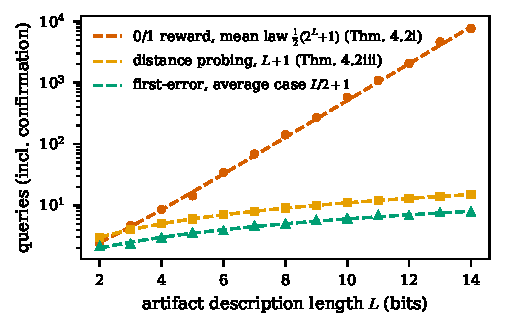
\includegraphics[width=0.96\textwidth]{figures/fig_feedback.pdf}
\caption{Feedback separation (Thms.~\ref{thm:fano}--\ref{thm:separation}). Mean queries to identify an $L$-bit target, \emph{each protocol executed as an algorithm} (60 runs; markers), vs.\ exact laws (dashed): scalar mean hitting law $(2^L{+}1)/2$; distance probing's deterministic $L{+}1$; first-error's \emph{average case} $L/2{+}1$ under the confirming-query convention (Thm.~\ref{thm:separation}(ii) bounds identification by $L$).}
\label{fig:feedback}
\end{minipage}\hfill
\begin{minipage}[t]{0.48\textwidth}
\centering
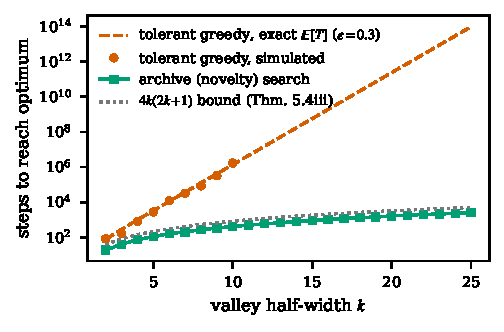
\includegraphics[width=0.96\textwidth]{figures/fig_deception.pdf}
\caption{Deception separation (Thm.~\ref{thm:deception}) on the unique-optimum landscape ($f(2k) = 2k > k = f(0)$). Steps to cross a valley of half-width $k$: tolerant greedy ($\eps = 0.3$; exact and simulated) grows exponentially; archive search stays under $4k(2k+1)$. Strict greedy never arrives (not plottable).}
\label{fig:deception}
\end{minipage}
\end{figure}

One audit note: an earlier draft reported the gated count in Figure~\ref{fig:ratchet}b as ``zero'' from this single seed; the theory's own Poisson prediction is $\approx 1.6$, and replaying the seed finds 2---a one-seed illusion caught by the paper's own theorem. Appendix~\ref{app:exp} has parameters, conventions, and verification printouts.

\section{Related Work}
\label{sec:related}

\textbf{Empirical beyond-gradient systems.} Prompt optimization spans APE, OPRO, PromptBreeder, and program-level compilers \citep{zhou2023ape, yang2024opro, fernando2023promptbreeder, khattab2024dspy, opsahlong2024mipro}, culminating in trace-reflective methods \citep{agrawal2025gepa, yuksekgonul2024textgrad, cheng2024trace}; context/memory evolution \citep{zhang2025ace, packer2023memgpt, suzgun2025cheatsheet}; skills and heuristics \citep{yang2026skillopt, weng2026hl}; agent/harness search \citep{hu2025adas, zhang2025dgm, lee2026metaharness}; code and discovery loops \citep{romeraparedes2024funsearch, novikov2025alphaevolve, karpathy2026autoresearch}; self-referential variants \citep{zelikman2024stop}. We add no system; we add the common load-bearing mathematics.

\textbf{Evaluation statistics.} The selection results of \S\ref{sec:ratchet} are the artifact-search reading of an archival literature on fictitious improvement under noisy evaluation: seed sensitivity in deep RL \citep{henderson2018matters}, expected-max inflation across tuning trials \citep{dodge2019show}, interval-based reporting \citep{agarwal2021precipice}. Our contribution is the closed-form ratchet law, the matching certification cost, and their composition with search (Theorem~\ref{thm:composed}).

\textbf{Theory.} Our prior-mass results adapt universal search \citep{levin1973universal, schmidhuber2004oops, hutter2005universal} and its agentic reading \citep{achille2025universal}. The feedback results are worst-case companions to the transfer-eluder theory \citep{xu2025llf, cheng2023llfbench}, against the scalar-sufficiency position of \citet{silver2021reward}: scalars suffice in the limit, traces change the \emph{rate}. Selection-under-noise imports best-arm identification \citep{evendar2006action, karnin2013almost, li2017hyperband}; deception, quality-diversity theory \citep{lehman2011abandoning, mouret2015illuminating} and runtime analysis \citep{droste2002analysis}; generalization, MDL/PAC-Bayes \citep{rissanen1978modeling, mcallester1999pac}; limits, No Free Lunch \citep{wolpert1997no} and Goodhart taxonomies \citep{manheim2018categorizing, amodei2016concrete}. Methodologically we follow the settle-the-question genre of \citet{bowling2023settling} and \citet{richens2025general}.

\section{Discussion and Conclusion}
\label{sec:discussion}

Definition~\ref{def:as} reduces the design space to five measurable quantities---cold prior mass $q_0(G_\eps)$, trace boost $\gamma$, feedback information, noise--gap ratio $\sigma^2/\Delta^2$, description length $\len(a)$---plus an evaluator-integrity condition; Theorem~\ref{thm:composed} shows the statistical dials multiply into one certified cost. Each result is a falsifiable scaling claim: hitting time inversely in measured prior mass; $\gamma$ estimable at known cost; scalar-vs-trace gaps in the feedback's usable bits; repeats as $(\sigma^2/\Delta^2)\log B$; generalization gaps as $\sqrt{\len(a)/n}$ (measurement designs: Appendix~\ref{app:extended}). \emph{Limitations:} the proposer is a fixed measure and the task stationary; the model does not explain \emph{why} LLM priors align with useful edits; the constructions are minimal worst cases; the mapping to deployed systems remains qualitative---no experiment here measures the dials live (Appendix~\ref{app:protocol}). \emph{Conclusion:} learning beyond gradients is stochastic program search with a learned prior, wide feedback, statistical selection, and description-length generalization---composing, when gated, into certified improvement at a compound rate.

\subsubsection*{Ethics statement}
This paper advances the theoretical understanding of self-improving LLM systems. Sharper theory for when such loops are sound (Corollary~\ref{cor:budget}, Theorem~\ref{thm:composed}, Proposition~\ref{prop:goodhart}) primarily supports safer engineering: it gives auditable conditions under which claimed autonomous improvements are real, and bounds on proxy gaming. The same analysis could marginally inform attempts to build more capable self-improving systems; we judge the safety-relevant clarity---particularly the evaluator-integrity condition---to outweigh this, and we discuss failure modes throughout rather than in isolation.

\subsubsection*{Reproducibility statement}
All proofs are self-contained in Appendices~\ref{app:prior}--\ref{app:goodhart} with explicit constants. All simulations are pure NumPy, seeded, and complete in under a minute on one CPU core (Appendix~\ref{app:exp}); the committed script regenerates every figure and prints every numeric claim made in \S\ref{sec:ratchet} and \S\ref{sec:experiments} (realized median $3.39\sigma$; $H_{2000} = 8.18$ vs.\ simulated $8.30$; 2 gated false accepts against a Poisson prediction of $1.61$), so prose and artifacts can be audited against each other---an audit this revision itself benefited from. The $\gamma$-measurement protocol of Appendix~\ref{app:protocol} is specified to the level of prompts, sample sizes, and confidence intervals.

\bibliography{references}
\bibliographystyle{iclr2027_conference}

\newpage
\appendix

\section{Proofs for Section~\ref{sec:prior} (Prior Mass)}
\label{app:prior}

\begin{proof}[Proof of Theorem~\ref{thm:hitting}]
\textbf{(i)} With i.i.d.\ proposals, $T$ is geometric with success probability $p$: $\P(T > t) = (1-p)^t$, so $\E[T] = \sum_{t \ge 0} (1-p)^t = 1/p$. For the tail, $(1-p)^t \le e^{-pt} \le \delta$ once $t \ge \ln(1/\delta)/p$.

\textbf{(ii)} $T$ is a stopping time for the i.i.d.\ sequence $(a'_t)$: the event $\{T \ge t\} = \{a'_1 \notin G_\eps, \dots, a'_{t-1} \notin G_\eps\}$ is determined by the first $t-1$ proposals, hence independent of $c(a'_t)$. Since $\E[T] = 1/p < \infty$ and $\E[c(a'_1)] = \bar{c} < \infty$ with $c \ge 0$, Wald's identity \citep{wald1944cumulative} gives $\E\big[\sum_{t=1}^{T} c(a'_t)\big] = \E[T]\, \bar{c} = \bar{c}/p$.

\textbf{(iii)} Let $p_t = q(G_\eps \mid a_t, y_t, \M_t)$ be the conditional hit probability at step $t$, so $p_t \ge \gamma\, q_0(G_\eps) \eqqcolon p_\gamma$ almost surely. Then
\[
\P(T > t) = \E\Big[\textstyle\prod_{i=1}^{t} (1 - p_i)\Big] \le (1 - p_\gamma)^t ,
\]
by iterated conditioning (peel off the last factor: $\E[\prod_{i \le t}(1-p_i)] = \E[\prod_{i \le t-1}(1-p_i)\,\E[(1-p_t) \mid \mathcal{F}_{t-1}]] \le (1-p_\gamma)\,\E[\prod_{i \le t-1}(1-p_i)]$, and induct). Summing the tail gives $\E[T] \le 1/p_\gamma$. If the boost holds only after $t_0$, bound the first $t_0$ steps by $t_0$ and apply the argument to the remainder.
\end{proof}

\begin{proof}[Proof of Proposition~\ref{prop:hitlower}]
By the union bound and iterated conditioning, $\P(T \le t) \le \sum_{i=1}^{t} \E[p_i] \le t \bar{q}$. Hence, with $m = \lfloor 1/\bar{q} \rfloor$,
\[
\E[T] = \sum_{t \ge 0} \P(T > t) \ge \sum_{t=0}^{m-1} \big(1 - t\bar{q}\big)
= m - \bar{q}\,\frac{m(m-1)}{2} \ge m - \frac{m}{2} = \frac{m}{2} \ge \frac{1}{2\bar{q}} - 1 .
\]
(The second inequality uses $\bar q (m-1) \le 1$.)
\end{proof}

\begin{proof}[Proof of Remark~\ref{rem:misleading}]
If the conditional mass equals $\gamma q_0(G_\eps)$ at every step, the indicator of a hit at each step is Bernoulli$(\gamma q_0(G_\eps))$ conditionally on the past, so $\P(T > t) = (1 - \gamma q_0(G_\eps))^t$ exactly and $\E[T] = 1/(\gamma q_0(G_\eps))$, which exceeds the cold rate $1/q_0(G_\eps)$ iff $\gamma < 1$. Under the one-sided hypothesis with $\bar q = \gamma q_0(G_\eps)$, Proposition~\ref{prop:hitlower} gives $\E[T] \ge 1/(2\gamma q_0(G_\eps)) - 1$, which exceeds $1/q_0(G_\eps)$ iff $\gamma < 1/\big(2(1 + q_0(G_\eps))\big)$; for $\gamma$ between this threshold and $1$ the one-sided hypothesis alone is silent, which is why the prose claim in \S\ref{sec:prior} is stated through the exact-mass version.
\end{proof}

\begin{proof}[Proof of Proposition~\ref{prop:gammaest}]
Write $q_0 = q_0(G)$, $q_\tau = q_\tau(G)$, and $e_K = \sqrt{\ln(4/\delta)/(2K)}$. Each empirical pass rate is a mean of $K$ i.i.d.\ Bernoulli variables, so Hoeffding's inequality \citep{hoeffding1963probability} gives $\P(|\hat q_0 - q_0| \ge e_K) \le 2e^{-2Ke_K^2} = \delta/2$ and likewise for $\hat q_\tau$; on the intersection (probability $\ge 1 - \delta$) both estimates are within $e_K$ of their means. The sample-size condition is exactly $e_K \le \eta\, q_{\min}/3$; write $x = \eta/3 \le 1/3$. Since $q_0, q_\tau \ge q_{\min}$, we have $e_K/q_0 \le x$ and $e_K/q_\tau \le x$, and $\hat q_0 \ge q_0 - e_K \ge (1-x)q_{\min} > 0$, so $\hat\gamma$ is well defined. Then
\[
\hat\gamma \;\le\; \frac{q_\tau + e_K}{q_0 - e_K} \;=\; \gamma\,\frac{1 + e_K/q_\tau}{1 - e_K/q_0} \;\le\; \gamma\,\frac{1+x}{1-x} \;\le\; \gamma\,(1 + 3x) \;=\; \gamma(1+\eta),
\]
using $(1+x)/(1-x) \le 1 + 3x$ for $x \le 1/3$; and symmetrically
$\hat\gamma \ge \gamma\,(1-x)/(1+x) \ge \gamma(1 - 2x) \ge \gamma(1 - \eta)$.
\end{proof}

\section{Proofs for Section~\ref{sec:feedback} (Feedback Information)}
\label{app:feedback}

\begin{proof}[Proof of Theorem~\ref{thm:fano}]
First take the algorithm deterministic. Its behavior is a decision tree: the query at round $t+1$ is a fixed function of the transcript $(y_1, \dots, y_t) \in \Y^t$, and the final output is a fixed function of $(y_1, \dots, y_T)$. Run the algorithm against every $a^* \in \A^*$. The number of distinct realizable transcripts of length $T$ is at most $|\Y|^T$, so the final-output map takes at most $|\Y|^T$ distinct values. Similarly, the query asked at round $t+1$ is determined by a transcript prefix in $\Y^{t}$, so over all rounds and all runs the set of artifacts ever queried has size at most $\sum_{t=0}^{T-1} |\Y|^{t} \le 2 |\Y|^T$ for $|\Y| \ge 2$.

Credit the algorithm with success if it ever queries $a^*$ or outputs $a^*$ (this is generous). The set $S$ of targets on which it can succeed therefore satisfies $|S| \le |\Y|^T + 2|\Y|^T = 3|\Y|^T$. For uniform $a^*$,
\[
\tfrac{1}{2} \le \P(\text{success}) = \frac{|S|}{2^L} \le \frac{3 |\Y|^T}{2^L}
\quad\Longrightarrow\quad
|\Y|^T \ge \frac{2^L}{6}
\quad\Longrightarrow\quad
T \ge \frac{L - \log_2 6}{\log_2 |\Y|} .
\]
A randomized algorithm is a mixture over deterministic ones (condition on the random seed); since the success probability is the mixture average, some deterministic realization succeeds with probability $\ge 1/2$, and the bound applies to it. (Fano-type arguments of this form are standard; see \citealp{cover2006elements}.)
\end{proof}

\begin{proof}[Proof of Theorem~\ref{thm:separation}]
\textbf{(i)} Until the needle is hit, every response equals $0$, so a deterministic algorithm's queries form a fixed sequence $b_1, b_2, \dots$ (repetitions only hurt; assume distinct). The hitting round is the position of $a^*$ in this sequence. For uniform $a^*$ over $2^L$ artifacts, $\E[T] = \sum_{j=1}^{2^L} j \cdot 2^{-L} = (2^L+1)/2$ when the sequence enumerates $\A^*$, and is larger otherwise. Averaging over the seed extends this to randomized algorithms.

\textbf{(ii)} Maintain a current string $a$, initialized arbitrarily. Query $a$; if correct, done; otherwise the feedback names the first index $i$ where $a_i \ne a^*_i$. Flip $a_i$. This flip makes coordinate $i$ correct and does not alter coordinates $j < i$, which were already correct (the first error was at $i$). Hence the length of the correct prefix increases strictly with each query, and at most $L$ queries are needed to know $a^*$; a further confirming query observes the success response if the protocol requires it.

\textbf{(iii)} Query a base string $a^0$ and record $d_0 = d_H(a^0, a^*)$. For $i = 1, \dots, L$ query $a^0 \oplus e_i$: the distance is $d_0 - 1$ if coordinate $i$ of $a^0$ is wrong and $d_0 + 1$ if it is right. After $L+1$ queries every coordinate's correctness is known, determining $a^*$ exactly.
\end{proof}

\section{Proofs for Section~\ref{sec:selection} (Noise)}
\label{app:noise}

\begin{proof}[Proof of Theorem~\ref{thm:ratchet}]
\textbf{(i) Upper bound.} For any $\lambda > 0$, by Jensen's inequality and the subgaussian moment-generating bound $\E[e^{\lambda \hat{s}_i}] \le e^{\lambda^2\sigma^2/2}$,
\[
e^{\lambda \E[m_t]} \le \E[e^{\lambda m_t}] \le \sum_{i=1}^{t} \E[e^{\lambda \hat{s}_i}] \le t\, e^{\lambda^2 \sigma^2 / 2}
\;\;\Longrightarrow\;\;
\E[m_t] \le \frac{\ln t}{\lambda} + \frac{\lambda \sigma^2}{2},
\]
and choosing $\lambda = \sqrt{2 \ln t}/\sigma$ yields $\E[m_t] \le \sigma \sqrt{2 \ln t}$.

\textbf{(i) Lower bound (Gaussian case).} Fix $\eta \in (0,2)$ and set $x_t = \sqrt{(2-\eta)\ln t}$. Using the Gaussian tail bound $1 - \Phi(x) \ge \frac{x}{1+x^2}\,\varphi(x)$,
\[
t\,\big(1 - \Phi(x_t)\big) \;\ge\; t \cdot \frac{x_t}{1+x_t^2} \cdot \frac{e^{-x_t^2/2}}{\sqrt{2\pi}}
\;=\; \frac{x_t}{(1+x_t^2)\sqrt{2\pi}} \; t^{\eta/2} \;\xrightarrow[t \to \infty]{}\; \infty .
\]
Hence $\P(m_t/\sigma \le x_t) = \Phi(x_t)^t \le \exp\{-t(1-\Phi(x_t))\} \to 0$. Since $m_t \ge \hat{s}_1$ pointwise, $\E[m_t \mathbf{1}\{m_t \le \sigma x_t\}] \ge -\E|\hat{s}_1| \ge -\sigma\sqrt{2/\pi}$, so
\[
\E[m_t] \ge \sigma x_t \,\P(m_t > \sigma x_t) - \sigma\sqrt{2/\pi} = (1-o(1))\,\sigma\sqrt{(2-\eta) \ln t}.
\]
Letting $\eta \downarrow 0$ along $t \to \infty$ gives the claim. The second-order correction is negative---for Gaussian maxima the median sits $\approx (\ln\ln t + \ln 4\pi)/(2\sqrt{2\ln t})$ \emph{below} $\sigma\sqrt{2\ln t}$ \citep{boucheron2013concentration}---which is the visible gap in Figure~\ref{fig:ratchet}a and the reason the realized $t = 2000$ median is $3.39\sigma$ rather than $3.90\sigma$.

\textbf{(ii)} Under the empty-incumbent convention, the $i$-th candidate is accepted iff $\hat{s}_i > \max_{j < i} \hat{s}_j$, i.e.\ iff $\hat s_i$ is a \emph{record}. For i.i.d.\ draws from a continuous distribution, each of the first $i$ values is equally likely to be the largest, so $\P(\hat{s}_i \text{ is a record}) = 1/i$, and linearity of expectation gives $\E[\#\text{accepts up to } t] = H_t$. Under the measured-incumbent convention the relevant sequence is $(\hat s_0, \hat s_1, \dots, \hat s_t)$ and candidate $i \ge 1$ is accepted iff it is a record of that extended sequence, with probability $1/(i+1)$; summing gives $H_{t+1} - 1$. (With atoms, ties only reduce records.)
\end{proof}

\begin{proof}[Proof of Proposition~\ref{prop:repeats}]
\textbf{(i) Two-sided gate.} Estimate each side by an average of $N$ fresh evaluations and let $\widehat{D}$ be the difference; $\widehat{D} - D$ is a sum of $2N$ independent $\sigma$-subgaussian terms scaled by $1/N$, hence $\sqrt{2/N}\,\sigma$-subgaussian. The rule ``accept iff $\widehat{D} \ge \Delta/2$'' errs only if $|\widehat{D} - D| \ge \Delta/2$ (under either hypothesis $D = 0$ or $D = \Delta$), which has probability at most $\exp\{-(\Delta/2)^2 / (2 \cdot 2\sigma^2/N)\} = \exp\{-N\Delta^2/(16\sigma^2)\} \le \delta$ for $N \ge (16\sigma^2/\Delta^2)\ln(1/\delta)$.

\textbf{(ii) Lower bound.} A decision rule with both errors $\le \delta$ is a test between $P_0 = \mathcal{N}(0, \sigma^2)^{\otimes N}$ and $P_1 = \mathcal{N}(\Delta, \sigma^2)^{\otimes N}$ (the hardest noise instance consistent with the model). By the Bretagnolle--Huber inequality \citep{tsybakov2009introduction}, the sum of the two error probabilities of any test satisfies
\[
2\delta \;\ge\; \tfrac{1}{2}\, e^{-\mathrm{KL}(P_0, P_1)} \;=\; \tfrac{1}{2}\, e^{-N\Delta^2/(2\sigma^2)}
\quad\Longrightarrow\quad
N \;\ge\; \frac{2\sigma^2}{\Delta^2} \ln \frac{1}{4\delta},
\]
nonvacuous for $\delta < 1/4$. (The constant $\ln(1/(4\delta))$ is what the argument yields; an earlier version of this paper stated $\ln(1/(2\delta))$, which is stronger than proven.)

\textbf{(iii) One-sided gate.} The candidate's $N$-evaluation mean $M$ satisfies: $M - \mu_{\mathrm{cand}}$ is $\sigma/\sqrt{N}$-subgaussian. Accept iff $M \ge \mu_{\mathrm{inc}} + \Delta/2$, where $\mu_{\mathrm{inc}}$ is the known incumbent mean. If the true gain is $\le 0$, acceptance requires $M - \mu_{\mathrm{cand}} \ge \Delta/2$; if the true gain is $\ge \Delta$, rejection requires $\mu_{\mathrm{cand}} - M \ge \Delta/2$. Either event has probability at most $\exp\{-(\Delta/2)^2/(2\sigma^2/N)\} = \exp\{-N\Delta^2/(8\sigma^2)\} \le \delta$ for $N \ge (8\sigma^2/\Delta^2)\ln(1/\delta)$.
\end{proof}

\begin{proof}[Proof of Corollary~\ref{cor:budget}]
Apply Proposition~\ref{prop:repeats}(i) (resp.\ (iii)) with confidence $\delta' = \delta/B$ to each of the $B$ decisions and take a union bound over the run. The per-decision cost is $N = \lceil (16\sigma^2/\Delta^2) \ln(B/\delta) \rceil$ (resp.\ $\lceil (8\sigma^2/\Delta^2) \ln(B/\delta) \rceil$).
\end{proof}

\section{Proofs for Section~\ref{sec:selection} (Deception)}
\label{app:deception}

\begin{proof}[Proof of Theorem~\ref{thm:deception}]
\textbf{(i)} At state $0$, the proposal is $-1$ (rejected as out of range; the walk stays) or $1$, and $f(1) = k - 1 < k = f(0)$, so a strict-improvement rule rejects it; the chain remains at $0$ forever, and $f(0) = k < 2k = f(2k)$. (From any start in $[1, k]$, only leftward moves are improvements, so the walk descends to $0$ and then halts.)

\textbf{(ii)} In the valley interior $i \in [1, k-1]$, a step proposes left or right with probability $1/2$ each; the left move is improving (always accepted), the right move is worsening (accepted with probability $\eps$). Thus the per-step transition probabilities are $p = \eps/2$ (right), $q = 1/2$ (left), and stay otherwise. At $i = 0$, $p = \eps/2$ and $q = 0$ (the left proposal is rejected as out of range). On the ascent $i \in (k, 2k)$, the right move is improving since $f$ is increasing there ($p = 1/2$) and the left move worsens ($q = \eps/2$); at the floor $i = k$ both neighbors improve ($p = q = 1/2$). Note these probabilities---and hence all hitting times---are identical to those of the symmetric-slope landscape: the asymmetric ascent changes $f$-values, not accept/reject comparisons. Let $h_i$ be the expected time to first reach $i+1$ from $i$. First-step analysis for $i \ge 1$ in the valley:
\[
h_i = 1 + q\,(h_{i-1} + h_i) + (1 - p - q)\,h_i
\;\;\Longrightarrow\;\;
h_i = \frac{1 + q\, h_{i-1}}{p} = \frac{2}{\eps} + \frac{1}{\eps}\, h_{i-1},
\qquad h_0 = \frac{2}{\eps},
\]
where $h_0 = 2/\eps$ reflects the stated boundary convention (the proposal at $0$ is right with probability $1/2$ and accepted with probability $\eps$). By induction $h_i \ge \eps^{-i} h_0 = 2\,\eps^{-(i+1)}$. The time to reach $2k$ from $0$ is at least the time to first reach $k$, which is $\sum_{i=0}^{k-1} h_i \ge h_{k-1} \ge 2\,\eps^{-k}$.

\textbf{(iii)} Let $r_t \le 2k$ be the rightmost element of the archive at step $t$ ($r_0 = 0$), and note the archive size never exceeds $2k+1$. While $r_t < 2k$, the step extends the frontier ($r_{t+1} = r_t + 1$) whenever the sampler picks the archive element $r_t$ (probability $\ge 1/(2k+1)$) and proposes its right neighbor (probability $1/2$; $r_t+1$ is not in the archive by maximality of $r_t$). Hence each frontier advance is stochastically dominated by a geometric random variable with success probability $1/(2(2k+1))$, and $2k$ advances are needed:
\[
\E[T] \;\le\; 2k \cdot 2(2k+1) \;=\; 4k(2k+1).
\]
The rule never consults $f$, so deception is irrelevant to it; it pays instead in evaluations of artifacts that are currently worse, which is the quantitative trade championed by novelty search \citep{lehman2011abandoning}.
\end{proof}

\begin{remark}
The constants in (ii) are not optimized; any acceptance rule whose probability of accepting a worsening move is at most $\eps$ obeys the same bound, including Metropolis rules at fixed temperature \citep{kirkpatrick1983optimization}. Birth--death hitting-time formulas are classical \citep{levin2017markov}. The exact expectation plotted in Figure~\ref{fig:deception} sums $h_i$ over the full chain including the ascent segment.
\end{remark}

\section{Proof for Section~\ref{sec:composition} (Composition)}
\label{app:composed}

\begin{proof}[Proof of Theorem~\ref{thm:composed}]
Throughout, a \emph{decision} at step $t$ consists of drawing a candidate $a'_t \sim q(\cdot \mid a_t, y_t, \M_t)$, drawing $N$ fresh evaluations of $a'_t$ and $N$ of the incumbent $a_t$ (evaluation noise independent of everything previous), and accepting iff the measured gain is $\ge \Delta/2$. Write $D_t = F(a'_t) - F(a_t)$ for the true gain and let $\mathcal{F}_{t-1}$ denote the history up to and including decision $t-1$ (proposals, evaluations, gate outcomes).

\emph{Gate error bounds.} Conditioning on $(a'_t, a_t)$, the proof of Proposition~\ref{prop:repeats}(i) gives, for the chosen $N = \lceil (16\sigma^2/\Delta^2)\ln(B/\delta) \rceil$:
\[
\P(\text{accept} \mid D_t \le 0) \;\le\; e^{-N\Delta^2/(16\sigma^2)} \;\le\; \frac{\delta}{B},
\qquad
\P(\text{reject} \mid D_t \ge \Delta) \;\le\; \frac{\delta}{B}.
\tag{$\ast$}
\]
Both directions come from the same Hoeffding bound: the measured gain deviates from $D_t$ by $\ge \Delta/2$ with probability at most $\delta/B$.

\emph{(i) Soundness.} A false accept at step $t$ is an acceptance with $D_t \le 0$. By ($\ast$) and a union bound over at most $B$ decisions, the probability of any false accept during the run is at most $\delta$. Call this good event $E_1$.

\emph{(ii) Liveness.} Let $T$ be the first decision at which a candidate in $G_\eps$ is accepted; we bound $T$ on a high-probability event. First observe that before such an acceptance the incumbent is never in $G_\eps$: $a_0 \notin G_\eps$ by hypothesis, and any accepted candidate either lies in $G_\eps$ (which would be the event in question) or does not (leaving the incumbent outside $G_\eps$). Therefore, at every decision $t \le T$, if the candidate lies in $G_\eps$ then $(\Delta,\eps)$-separation gives $D_t \ge \Delta$, and by ($\ast$) the gate accepts it with probability at least $1 - \delta/B$, using evaluation randomness independent of $\mathcal{F}_{t-1}$ and of the proposal draw. Combining with Assumption~\ref{ass:boost},
\[
\P\big(\text{decision } t \text{ accepts some } a \in G_\eps \,\big|\, \mathcal{F}_{t-1},\, T > t-1\big)
\;\ge\; \pgam \big(1 - \tfrac{\delta}{B}\big) \;\eqqcolon\; \rho .
\]
By the peel-the-last-factor induction of Theorem~\ref{thm:hitting}(iii), $\P(T > t) \le (1-\rho)^t \le e^{-\rho t}$, whence $\E[T] \le 1/\rho$ and $\P\big(T > \ln(1/\delta)/\rho\big) \le \delta$. Since $\delta \le \tfrac12$ and $B \ge 1$ give $\delta/B \le \tfrac12$, we have $\rho \ge \pgam/2$, so $T \le \lceil 2\ln(1/\delta)/\pgam \rceil$ with probability $\ge 1 - \delta$; the hypothesis $B \ge 2\ln(1/\delta)/\pgam$ ensures the run is long enough. Call this good event $E_2$.

\emph{(iii) Cost, and conclusion.} On $E_1 \cap E_2$, which has probability $\ge 1 - 2\delta$ by the union bound, both (i) and (ii) hold, and the number of evaluator calls up to the certifying acceptance is at most $2N$ per decision times $T$ decisions:
\[
2NT \;\le\; 2\,\Big\lceil \tfrac{16\sigma^2}{\Delta^2}\ln\tfrac{B}{\delta} \Big\rceil \cdot \Big\lceil \tfrac{2\ln(1/\delta)}{\pgam} \Big\rceil
\;=\; O\!\left( \frac{\sigma^2}{\Delta^2} \cdot \frac{\ln(B/\delta)\,\ln(1/\delta)}{\gamma\, q_0(G_\eps)} \right). \qedhere
\]
\end{proof}

\begin{remark}
The argument uses Assumption~\ref{ass:boost} in exactly the form stated: almost surely over \emph{all} histories, which in a gated run include accept/reject outcomes; this is what lets the boost survive the conditioning introduced by the gate. If incumbents are certified once and their means treated as known thereafter, Proposition~\ref{prop:repeats}(iii) halves the constant ($8$ for $16$) and the evaluator cost in (iii) drops to $NT$.
\end{remark}

\section{Proofs for Section~\ref{sec:compression} (Generalization)}
\label{app:occam}

\begin{proof}[Proof of Theorem~\ref{thm:occam}]
Per-instance scores lie in $[0,1]$, so for fixed $a$, Hoeffding's inequality \citep{hoeffding1963probability} gives $\P(|F(a) - \Fhat_n(a)| \ge t) \le 2e^{-2nt^2}$. Set $t_a = \sqrt{(\len(a)\ln 2 + \ln(2/\delta))/(2n)}$ and union over $\A$:
\[
\P\Big(\exists a : |F(a) - \Fhat_n(a)| \ge t_a\Big)
\;\le\; \sum_{a \in \A} 2 e^{-2n t_a^2}
\;=\; \sum_{a \in \A} 2 \cdot 2^{-\len(a)} \cdot \frac{\delta}{2}
\;\le\; \delta,
\]
using the Kraft inequality $\sum_a 2^{-\len(a)} \le 1$ for prefix-free codes. The guarantee is simultaneous over $\A$, so it covers any data-dependent selection $\hat{a}$, however adaptive.
\end{proof}

\begin{proof}[Proof of Corollary~\ref{cor:ushape}]
Let $a^\star_L$ attain $\max_{\len(a) \le L} F(a)$ and let $\eps_L = \sqrt{(L \ln 2 + \ln(2/\delta))/(2n)}$. On the event of Theorem~\ref{thm:occam}, every $a$ with $\len(a) \le L$ has $|F(a) - \Fhat_n(a)| \le \eps_L$. Hence
\[
F(\hat{a}_L) \ge \Fhat_n(\hat{a}_L) - \eps_L \ge \Fhat_n(a^\star_L) - \eps_L \ge F(a^\star_L) - 2\eps_L ,
\]
and $\sup_a F - F(\hat a_L) \le \big(\sup_a F - F(a^\star_L)\big) + 2\eps_L = A(L) + 2\eps_L$.
\end{proof}

\section{Proofs for Section~\ref{sec:limits} (Proxy Gaps)}
\label{app:goodhart}

\begin{proof}[Proof of Proposition~\ref{prop:goodhart}]
\textbf{(i)} $F(a_T) - F(a_0) = \big(\Ftil(a_T) - \Ftil(a_0)\big) - \big(b(a_T) - b(a_0)\big) \ge g - 2\alpha$.

\textbf{(ii)} For the upper bound, condition on the $F$-values and note $\Ftil(\hat a) - F(\hat a) = b(\hat a) \le \max_{i \le m} b_i$; the expected maximum of $m$ independent $\sigma_b$-subgaussian variables is at most $\sigma_b\sqrt{2\ln m}$ (the MGF argument of Theorem~\ref{thm:ratchet}(i)). When all $F(a_i)$ are equal and $b_i \sim \mathcal{N}(0, \sigma_b^2)$ i.i.d., $\hat a = \arg\max b_i$, and the Gaussian extreme-value lower bound from Appendix~\ref{app:noise} gives $\E[b(\hat a)] \ge (1-o(1))\,\sigma_b\sqrt{2 \ln m}$.

\textbf{(iii)} The construction stays inside the model. Take $\A = \{a_0, a_1, a_2, \dots\}$ with
\[
F(a_j) = 2^{-j} \in (0, 1], \qquad \Ftil(a_j) = 1 - 2^{-(j+1)} \in [\tfrac12, 1),
\]
so the bias is $b(a_j) = \Ftil(a_j) - F(a_j) = 1 - 3 \cdot 2^{-(j+1)}$, which grows along the path---the formal meaning of an evaluator that the loop edits as it goes (each step is a one-line ``relax the check'' edit, so the proposer places mass on $a_{j+1}$ from $a_j$). The proxy ratchet accepts every step since $\Ftil$ is strictly increasing; along the run, measured score rises to $1$ while true score falls from $F(a_0) = 1$ to $0$, traversing the full range. For the final claim: after $T$ steps the measured progress is $g_T = \Ftil(a_T) - \Ftil(a_0) = \tfrac12 - 2^{-(T+1)} \in (0, \tfrac12)$ while the true progress is $F(a_T) - F(a_0) = 2^{-T} - 1 \to -1$. Any transfer inequality $F\text{-progress} \ge \psi(\Ftil\text{-progress})$ with $\psi(g) > -1$ for some $g \in (0, \tfrac12)$ attained infinitely often is violated at large $T$; only the vacuous bound $\psi \equiv -1$ (the full range) survives. (Documented instances of the hypothesis: hallucinated tool logs \citep{zhang2025dgm}, simulator exploits in evolved rewards \citep{ma2024eureka}.)
\end{proof}

\section{Experimental Details and Audit Trail}
\label{app:exp}

All simulations are pure NumPy, seeded (\texttt{default\_rng(0)}), and complete in under a minute on one CPU core; the script \texttt{code/simulations.py} regenerates all figures and prints every numeric claim below. The RNG call order of the ratchet simulation is kept identical across revisions so that the seed-0 numbers are stable under audit.

\textbf{Ratchet (Fig.~\ref{fig:ratchet}).} $T = 2000$ null candidates, Gaussian noise $\sigma = 1$, $R = 400$ independent runs. Panel (a): median and 10--90\% band of $m_t$, against the $\sigma\sqrt{2\ln t}$ upper bound. Realized values at $t = 2000$: median $3.39\sigma$, mean $3.44\sigma$, against the bound's $3.90\sigma$; the deficit matches the second-order extreme-value correction $\approx (\ln\ln t + \ln 4\pi)/(2\sqrt{2\ln t}) \approx 0.5\sigma$. Panel (b): mean cumulative accepts ($8.30$ simulated at $t=2000$) vs.\ $H_{2000} = 8.18$. The gated variant implements the one-sided gate of Corollary~\ref{cor:budget}(ii)---appropriate here because the incumbent (null) mean is known to be $0$---with $N = \lceil 8\sigma^2 \ln(2000/0.05) \rceil = \lceil 84.77 \rceil = 85$ evaluations per candidate and threshold $\Delta/2$. Across the $400 \times 2000 = 8\times10^5$ gated decisions it accepted $2$ null edits: a per-run rate of $0.005$, within the $\delta = 5\%$ per-run certificate, and consistent with the exact per-candidate rate $p_N = \P(\mathcal{N}(0, 1/N) \ge \tfrac12) \approx 2.0\times10^{-6}$, i.e.\ a Poisson prediction of $\approx 1.61$ accepts in total. \emph{Audit note:} an earlier draft reported this count as ``zero across all runs,'' an artifact of reading a single seed's flat plot---in a paper about one-evaluation illusions, a one-seed illusion. The inset of Figure~\ref{fig:ratchet}b now shows the rate on a log scale instead of letting it render as exactly zero.

\textbf{Feedback (Fig.~\ref{fig:feedback}).} $L \in \{2, \dots, 14\}$, 60 runs per point; \emph{all three arms execute their algorithm}. Scalar: uniform search without replacement over an explicit random permutation of the $2^L$ candidates (mean hitting position $(2^L+1)/2$). First-error: the prefix-fixing algorithm of Theorem~\ref{thm:separation}(ii) from the all-zeros string, counting the final confirming query, hence average $\approx L/2 + 1$ for a uniform target (worst case $L+1$; identification per se uses $\le L$). Distance probing: the base-plus-flips scheme of Theorem~\ref{thm:separation}(iii), executed with a correctness assertion on the reconstructed target; deterministically $L+1$ queries.

\textbf{Deception (Fig.~\ref{fig:deception}).} $\eps = 0.3$; landscape $f(i) = k - i$ on $[0,k]$, $f(i) = 2(i-k)$ on $[k,2k]$ (unique optimum, Theorem~\ref{thm:deception}); proposals to $\{i-1,i+1\}$ uniformly, out-of-range rejected. Exact $\E[T]$ sums the first-step recurrences $h_i$ over the full chain $[0, 2k]$ including the ascent side ($p = 1/2$, $q = \eps/2$) and the valley floor ($p = q = 1/2$); the acceptance probabilities, hence the exact curve, are unchanged by the asymmetric slope. Verification printouts: exact-to-bound ratio $\E[T] / (2\eps^{-k}) \to 4.08$ at $k = 25$; archive means $111 / 420 / 2551$ at $k = 5/10/25$ against the $4k(2k+1)$ bounds $220 / 840 / 5100$. Simulation: tolerant greedy $k \le 10$, 12 runs per point (larger $k$ is computationally pointless given the exact curve); archive 60 runs per point, $k \le 25$.

\section{A Pre-Registered Protocol for Measuring the Trace Boost $\gamma$}
\label{app:protocol}

Proposition~\ref{prop:gammaest} reduces Assumption~\ref{ass:boost} to an estimation problem. The following protocol instantiates it at rebuttal scale; we state it concretely enough to be falsified.

\textbf{Task family.} $M = 120$ small Python functions, each with a single planted bug and a deterministic test suite (3--10 unit tests; e.g.\ curated from HumanEvalFix-style corpora or hand-written). The good set $G$ for each task is the set of patches under which all tests pass; membership is decided by the verifier (run the tests), not by any model.

\textbf{Conditions.} For each task, sample $K = 70$ independent patch proposals at temperature $1$ from one frozen open-weights model under two prompts that differ \emph{only} in feedback: (a) \emph{cold}: the buggy function and the name of the failing test; (b) \emph{trace}: additionally the full execution trace (stack trace, error message, failing assertion with values). Identical sampling parameters; no system-prompt differences beyond the feedback block.

\textbf{Estimates.} Per condition, the pooled pass rate $\hat q = (\#\text{passing proposals})/(MK)$ with a Wilson 95\% interval \citep{brown2001interval}, and the per-task rates for heterogeneity. The boost estimate is $\hat\gamma = \hat q_{\mathrm{trace}} / \hat q_{\mathrm{cold}}$ with the interval ratio; Proposition~\ref{prop:gammaest} gives the a-priori sample-size certificate: certifying $\gamma$ within a factor of two ($\eta = 1$) at $q_{\min} = 0.05$, $\delta = 0.05$ requires $\tfrac{9}{2 q_{\min}^2}\ln 80 \approx 7.9 \times 10^3$ verified proposals per condition, covered by the $MK = 8.4\times10^3$ budget (Hoeffding is conservative; Wilson intervals are tighter in practice). Tasks with $\hat q_{\mathrm{cold}} = 0$ are reported separately as cold-unsolvable.

\textbf{Outcomes.} The framework predicts $\hat\gamma$ substantially above $1$, with task-level $\hat\gamma$ correlating with trace informativeness; Theorem~\ref{thm:hitting}(iii) then converts $\hat\gamma$ into a hitting-time prediction checkable against the same logs. The falsifying outcome is an interval for $\hat\gamma$ containing $1$: Assumption~\ref{ass:boost} would then be doing no work on this family, and the paper's adaptive story would need revision. Total cost is roughly $1.7\times10^4$ generations plus test executions---about one GPU-day with a small open model.

\textbf{Scaling up.} The same design lifts to harness search for web agents, where regenerable environments with per-task verifiers supply the fresh, repeatable evaluator the theory requires \citep{zhou2024webarena}: conditions become harness variants with and without execution-history feedback, and $G$ is task success under the benchmark verifier.

\section{The Open Problem: Rates for Self-Reference}
\label{app:open}

Let an outer loop optimize an artifact that is itself an optimizer (STOP's improver, PromptBreeder's mutation prompts, the DGM's self-modifications), and let $\alpha_t$ denote the evaluator gap $\sup |b|$ at round $t$ while $m_t$ denotes the optimization pressure (candidates considered per round). Proposition~\ref{prop:goodhart}(ii) suggests the harvested bias grows like $\sigma_b\sqrt{2 \ln m_t}$ while (i) caps transferable progress at $g_t - 2\alpha_t$. \textbf{Open problem:} give natural conditions on the rates $(\alpha_t, m_t, g_t)$---evaluator re-estimation on fresh data vs.\ pressure growth---under which the self-referential ratchet converges to true improvement rather than Goodhart divergence, and matching impossibility results. Even the one-level version is open in the form stated: the bandit literature controls $\alpha_t$ by design, and the RSI literature \citep{yampolskiy2015seed, chalmers2010singularity, schmidhuber2003godel} discusses the limit without rates. We conjecture a phase transition at $\alpha_t = \Theta(\sigma_b \sqrt{\ln m_t})$.

\section{Extended System Mapping}
\label{app:mapping}

Table~\ref{tab:systems} compressed; here we record the fuller correspondence used in \S\ref{sec:model}--\S\ref{sec:limits}. Sources marked informal in Table~\ref{tab:systems} are used as illustrations only.

\begin{itemize}\itemsep2pt
\item \textbf{GEPA} \citep{agrawal2025gepa}: $\A$ = module prompts of a compound system; $y$ = full execution traces plus judge text; $\sel$ = per-instance Pareto frontier (Theorem~\ref{thm:deception}(iii)-style diversity preservation); minibatch gating (Proposition~\ref{prop:repeats} with small $N$); reported test-set degradation when validation is reused (Theorem~\ref{thm:occam} with growing $\len$, Proposition~\ref{prop:goodhart}(ii) with $m$ = candidates tried).
\item \textbf{SkillOpt} \citep{yang2026skillopt}: $\A$ = one skill document; bounded add/delete/replace edits (controlling $\len(a)$ growth, Corollary~\ref{cor:ushape}); strict held-out acceptance (fresh-data re-estimation, Proposition~\ref{prop:goodhart}(i)).
\item \textbf{ACE} \citep{zhang2025ace}: $\A$ = evolving context/playbook; documented \emph{context collapse} and \emph{brevity bias} are the two ends of Corollary~\ref{cor:ushape}'s U.
\item \textbf{Meta-Harness} \citep{lee2026metaharness}: $\A$ = executable harness; $y$ = raw prior code, traces, scores (maximal-information channel, \S\ref{sec:feedback}); long-horizon credit assignment over $\M$.
\item \textbf{autoresearch} \citep{karpathy2026autoresearch} (informal): $\A$ = training script; $\sigma$ large (5-minute proxy runs), single-evaluation greedy ratchet---an in-the-wild instance of Theorem~\ref{thm:ratchet}; reported surviving discoveries are those re-verified at higher $N$ (Corollary~\ref{cor:budget}). The archival grounding for this failure mode is \citet{henderson2018matters,dodge2019show,agarwal2021precipice}.
\item \textbf{Heuristic Learning} \citep{weng2026hl} (informal): $\A$ = executable heuristics; $y$ = logs/video replays; ``compress history'' = explicit $\len(a)$ control; reported failure on sparse-feedback exploration games = the misleading-feedback regime of Remark~\ref{rem:misleading}.
\item \textbf{ADAS / DGM} \citep{hu2025adas, zhang2025dgm}: $\A$ = agent programs; archives/lineages (Theorem~\ref{thm:deception}(iii)); the DGM paper's hallucinated-log episode (Proposition~\ref{prop:goodhart}(iii)).
\item \textbf{FunSearch / AlphaEvolve} \citep{romeraparedes2024funsearch, novikov2025alphaevolve}: $\A$ = programs; verified scalar evaluator ($\alpha = 0$, so Proposition~\ref{prop:goodhart}(i) is vacuous-strong and scalar feedback's slowness is paid in volume); island archives.
\item \textbf{Voyager} \citep{wang2023voyager}: additive skill library = monotone $\M$ growth re-weighting $q_0$ for later tasks (\S\ref{sec:prior}, reuse).
\item \textbf{Web-agent harness optimization} \citep{zhou2024webarena}: regenerable environments with per-task verifiers supply the fresh, low-$\alpha$, repeatable evaluator that Corollary~\ref{cor:budget} and Proposition~\ref{prop:goodhart}(i) require; the framework predicts harness search on such benchmarks is the most theory-compliant instance of the loop currently available, and Appendix~\ref{app:protocol} uses it as the scaled-up venue for the $\gamma$ measurement.
\end{itemize}

\section{LLM Usage Disclosure}
\label{app:llm}

In accordance with the ICLR policy on large language model usage: LLMs were used as general-purpose assistants for prose drafting, LaTeX preparation, and as coding assistants for the simulation scripts. All definitions, theorem statements, proofs, and numerical claims were checked by the authors; all simulation outputs regenerate deterministically from the committed seeded code, and the audit trail in Appendix~\ref{app:exp} documents one numerical prose error caught and corrected during revision. No LLM is an author, and the authors take full responsibility for all content.

\section{Extended Discussion: Predictions, Measurement Designs, and Outlook}
\label{app:extended}

The page limit forces the discussion of \S\ref{sec:discussion} to be compact; this appendix expands it without altering any claim. Each prediction below is a scaling law derived in the main text, paired with the experiment that would falsify it.

\paragraph{P1: Hitting time scales inversely with measured prior mass (Theorem~\ref{thm:hitting}).}
Fix a task family and harness; vary only the proposer (model scale, or base vs.\ instruction-tuned checkpoints of one family). Measure $\hat q_0(G_\eps)$ and $\hat\gamma$ by the Appendix~\ref{app:protocol} protocol, and independently measure realized hitting times of the full loop on held-out tasks. The prediction is a slope-$(-1)$ line of $\log \E[T]$ against $\log(\hat\gamma\,\hat q_0)$; systematic curvature would indicate history effects that Assumption~\ref{ass:boost} fails to absorb, and would localize exactly which conditioning the assumption misses.

\paragraph{P2: The scalar-vs-trace gap scales with the feedback's usable bits (Theorems~\ref{thm:fano}--\ref{thm:separation}).}
Degrade traces in controlled steps---full stack trace; error type and message only; failing-test name only; binary pass/fail---and measure proposals-to-fix on the same bug corpus. Theorem~\ref{thm:fano} prices each channel by $\log_2|\Y|$; Theorem~\ref{thm:separation} brackets the endpoints. The prediction is that identification cost interpolates monotonically between the $\le L$ and $\Omega(2^L)$ regimes as the channel narrows; a flat curve would mean the proposer cannot exploit the extra bits, separating channel capacity from usable information---itself a finding about $\gamma$.

\paragraph{P3: Required repeats scale as $(\sigma^2/\Delta^2)\log B$ (Proposition~\ref{prop:repeats}, Corollary~\ref{cor:budget}).}
In any ratchet-style optimizer, vary the per-evaluation budget (e.g.\ proxy-run length, which sets $\sigma$) and the acceptance margin $\Delta$, and count false accepts against a frozen ground-truth re-evaluation. The certified regime begins where Corollary~\ref{cor:budget} predicts; the experiment costs only logging, since the gate arithmetic is computed from measured $\hat\sigma$.

\paragraph{P4: Certified generalization gaps scale as $\sqrt{\len(a)/n}$ (Theorem~\ref{thm:occam}, Corollary~\ref{cor:ushape}).}
The cleanest missing measurement in this literature: instrument a deployed prompt optimizer to log, at every accepted step, the artifact's compressed length $\len(a)$ in bits, the validation size $n$, and the val--test gap on a fresh test set. Stratify gaps by evolved-prompt length. The prediction is the U-shape of Corollary~\ref{cor:ushape}: gaps growing like $\sqrt{\len(a)/n}$ on the right branch, task error dominating on the left, with the knee moving right as $n$ grows. Reports of validation overfitting in prompt evolution and of context collapse in context evolution \citep{zhang2025ace} are the two branches observed separately; no published study traverses the curve.

\paragraph{P5: Evaluator integrity is a phase boundary (Proposition~\ref{prop:goodhart}).}
In a sandboxed self-modification setting, compare matched loops in which the evaluator is (a) frozen and held out of the proposer's edit scope versus (b) reachable by edits. Proposition~\ref{prop:goodhart}(i)--(ii) predicts bounded, $\sqrt{2\ln m}$-degraded transfer in (a); (iii) predicts unbounded measured-vs-true divergence in (b). The qualitative version is documented (hallucinated logs, reward exploits); the quantitative boundary---how much evaluator surface area must be reachable before transfer fails---is open and measurable.

\paragraph{Limitations, expanded.}
Four boundaries of the model deserve more space than \S\ref{sec:discussion} can give them. \emph{Stationarity:} the task distribution $\D$ and evaluator are fixed; deployed loops face drift, and the certificates here say nothing about re-validation schedules under drift. \emph{Multi-objective artifacts:} real selectors (GEPA's instance-Pareto sets) optimize vector scores; our $F$ is scalar, and the deception analysis only gestures at why diversity preservation helps---a vector-valued treatment connecting Theorem~\ref{thm:deception} to Pareto-frontier maintenance is open. \emph{Interacting loops:} concurrent optimizers sharing an evaluator or a memory violate the single-trajectory model; their interference is unmodeled. \emph{Worst-case constructions:} the feedback and deception separations bound what is possible, not what is typical; bridging to instance-dependent rates---eluder-type quantities \citep{xu2025llf} measured on real systems---is the natural theoretical next step, just as the Appendix~\ref{app:protocol} measurement is the empirical one. Finally, the model is silent on \emph{why} LLM priors concentrate mass on useful edits; we import that fact from the in-context-learning literature \citep{xie2022explanation, akyurek2023what, vonoswald2023transformers, garg2022what} as an assumption made measurable, not explained.

\paragraph{Outlook.}
Naming the correspondence between the empirical systems and the five classical literatures buys the field what theory is for: successes become predictions, failures become theorems, and the next systems can be designed against bounds rather than anecdotes. The two measurements this paper specifies but does not run---the trace boost $\gamma$ (Appendix~\ref{app:protocol}) and the $(\len(a), n, \text{gap})$ curve (P4)---are where the framework is most exposed to data, and the open problem of Appendix~\ref{app:open} is where it is most exposed to mathematics.

\section{Notation}
\label{app:notation}

\begin{table}[h]
\centering
\small
\begin{tabular}{@{}lll@{}}
\toprule
Symbol & Meaning & Introduced \\
\midrule
$\A$, $a$, $a'$, $a^*$ & artifact space; artifact; candidate; target & Def.~\ref{def:as}, \S\ref{sec:feedback} \\
$F$, $\Fhat$, $\Fhat_n$ & true score; noisy evaluation; mean over $n$ validation instances & Def.~\ref{def:as}, Thm.~\ref{thm:occam} \\
$\Ftil = F + b$ & proxy score; $b$ its bias, $\alpha = \sup|b|$, $\sigma_b$ its subgaussian parameter & \S\ref{sec:limits} \\
$q$, $q_0$, $q_\tau$ & proposer; cold (unconditioned) proposer; trace-conditioned proposer & Def.~\ref{def:as}, Prop.~\ref{prop:gammaest} \\
$\gamma$, $\gamma_t$, $\hat\gamma$ & trace boost (Assumption~\ref{ass:boost}); its plug-in estimator & \S\ref{sec:prior} \\
$G_\eps$, $\eps$ & good set $\{a : F(a) \ge \sup F - \eps\}$; its tolerance & Def.~\ref{def:as} \\
$\pgam$ & $\gamma\, q_0(G_\eps)$, the boosted good-set mass & Thm.~\ref{thm:composed} \\
$T$ & hitting time (first proposal/acceptance in $G_\eps$, per context) & Def.~\ref{def:as} \\
$\sel$, $\M_t$ & selection rule; accumulated memory at step $t$ & Def.~\ref{def:as} \\
$y$, $\Y$, $\phi$ & feedback; feedback alphabet; feedback protocol & Def.~\ref{def:as}, \S\ref{sec:feedback} \\
$L$ & artifact bits (\S\ref{sec:feedback}); length budget (\S\ref{sec:compression}) & Thm.~\ref{thm:fano}, Cor.~\ref{cor:ushape} \\
$\sigma$, $\Delta$ & evaluation-noise subgaussian parameter; true-gain margin & \S\ref{sec:selection} \\
$\delta$, $B$, $N$ & confidence level; decision budget; evaluations per gated decision & Prop.~\ref{prop:repeats}, Cor.~\ref{cor:budget} \\
$m_t$, $H_t$ & running maximum of measured scores; harmonic number $\sum_{i\le t} 1/i$ & Thm.~\ref{thm:ratchet} \\
$\len(a)$, $A(L)$ & prefix-free description length; approximation error at length $L$ & \S\ref{sec:compression} \\
$k$ & valley half-width of the deception chain & Thm.~\ref{thm:deception} \\
$\eps$ (greedy) & acceptance probability of worsening moves in tolerant greedy & Thm.~\ref{thm:deception} \\
$m$ & number of candidates maximized over (optimizer's curse) & Prop.~\ref{prop:goodhart} \\
$K$, $q_{\min}$, $\eta$ & proposals per condition; good-mass lower bound; relative error & Prop.~\ref{prop:gammaest} \\
\bottomrule
\end{tabular}
\caption{Notation. The symbol $\eps$ is used for the good-set tolerance throughout and, locally in Theorem~\ref{thm:deception} only, for the tolerant-greedy acceptance probability; the two never co-occur.}
\label{tab:notation}
\end{table}

\end{document}
